\section{Dataset and Data Provenance}
\label{sec:data}

\textbf{Two public datasets, saved once and never edited.} Each experiment
\textbf{re-checks the SHA-256 fingerprint} and stops on a mismatch
(\repodir{data/raw}{raw data}, \repodir{data/cards}{dataset cards}).

\begin{table}[H]
\centering
\caption{Where the data came from and how many rows we use. Modelling rows exclude
the first \Warmup{} bars (feature windows not yet full) and the last bar (no next
close).}
\label{tab:dataset}
\small
\begin{tabular}{@{}L{0.20\linewidth} L{0.36\linewidth} L{0.36\linewidth}@{}}
\toprule
 & \textbf{Apple (AAPL)} & \textbf{Bitcoin (BTC/USDT)} \\
\midrule
\textbf{Source} & StockAnalysis public history API & Binance public REST API, spot \\
Endpoint & \scriptsize\url{https://stockanalysis.com/api/symbol/s/aapl/history} & \scriptsize\url{https://api.binance.com/api/v3/klines} \\
Fields & date, open, high, low, close, volume, adjusted close & open time, open, high, low, close, volume \\
\textbf{Window} & \WindowAAPL & \WindowBTC \\
Daily bars & \ObsAAPL & \ObsBTC \\
Quality checks$^{*}$ & \textbf{\QualityAAPL} & \textbf{\QualityBTC} \\
\textbf{Modelling rows} & \textbf{\RowsAAPL} & \textbf{\RowsBTC} \\
Train / validation / test & \TrainRowsAAPL{} / \ValidationRowsAAPL{} / \TestRowsAAPL & \TrainRowsBTC{} / \ValidationRowsBTC{} / \TestRowsBTC \\
\bottomrule
\end{tabular}
\par\smallskip\footnotesize
$^{*}$Duplicate dates, missing values, non-positive prices, inconsistent high, low or close, negative volume.
\end{table}

\begin{table}[H]
\centering
\caption{The two datasets differ. How we handled each difference.}
\label{tab:differences}
\small
\begin{tabular}{@{}L{0.16\linewidth} L{0.21\linewidth} L{0.19\linewidth} L{0.35\linewidth}@{}}
\toprule
Difference & AAPL & BTC & \textbf{What we did} \\
\midrule
Unit & listed share, USD & one exchange, USDT & Compare assets only by \textbf{unit-free skill} \\
Calendar & exchange sessions; \GapsAAPL{} weekend or holiday gaps & every day & Keep \textbf{each calendar}; never align rows \\
Close range & \CloseRangeAAPL & \CloseRangeBTC & Use \textbf{returns and ratios} as inputs \\
Daily volatility & \RetSdAAPL\% & \RetSdBTC\% & \textbf{Fit and score separately} \\
Adjusted price & differs on \AdjDiffPctAAPL\% of days & none & Predict the \textbf{raw close} \\
\bottomrule
\end{tabular}
\end{table}

Providers revise adjusted prices later, so they contain \textbf{information
unavailable at decision time}. No split discontinuity falls in the window (the
adjusted/raw ratio never jumps by more than 2\%), and we ignore dividends.

% Keep the generated split table here, in numbering order.
\begingroup
\let\floatingtable\table
\renewcommand{\table}[1][]{\floatingtable[H]}
% GENERATED by scripts/build_latex_assets.py -- do not edit by hand.
\begin{table}[t]
\centering
\caption{Chronological split boundaries in the asset's own calendar. One row is purged at each boundary so that no label crosses a split: with $y_t = C_{t+1}$, the last training label would otherwise be a validation price and the last validation label a sealed test price. The test block remains unopened.}
\label{tab:splits}
\small
\setlength{\tabcolsep}{4pt}
\begin{tabular}{@{}l l l l r@{}}
\toprule
Asset & Training & Validation & Sealed test & Total \\
\midrule
AAPL & 2021-12-10..2024-11-08 & 2024-11-12..2025-11-03 & 2025-11-05..2026-10-27 & 1,224 \\
BTC & 2021-11-27..2024-11-07 & 2024-11-09..2025-11-01 & 2025-11-03..2026-10-28 & 1,797 \\
\bottomrule
\end{tabular}
\par\smallskip\footnotesize
Total is the number of usable feature rows after the trailing-window warm-up and the terminal unlabelled row are removed.
\end{table}

\endgroup

\begin{figure}[t]
  \centering
  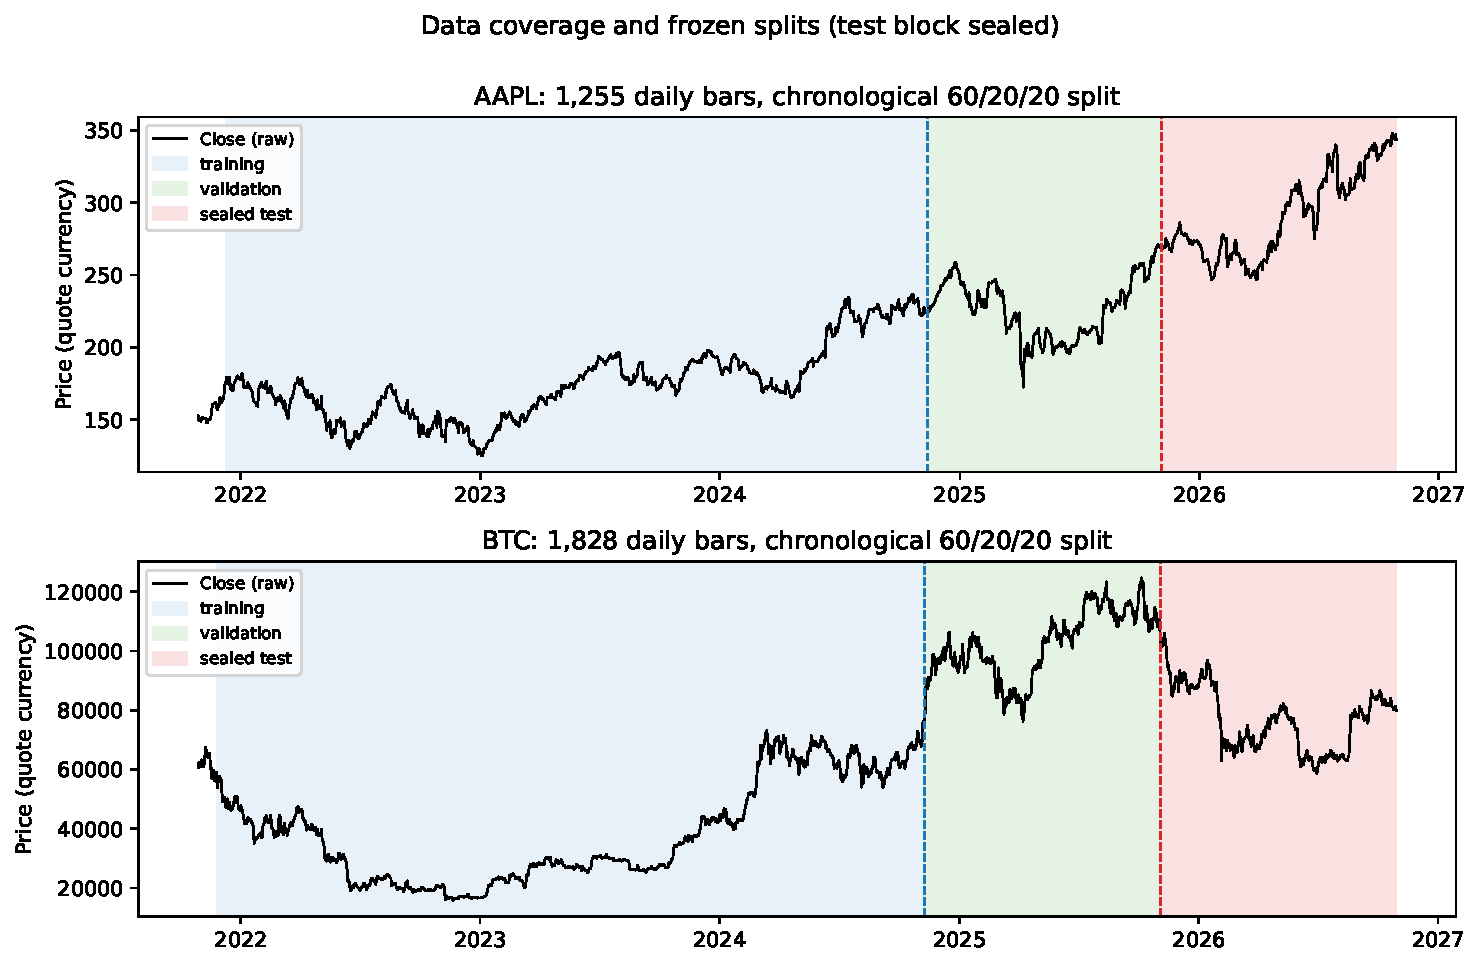
\includegraphics[width=0.9\linewidth]{figures/fig01_coverage_and_splits.pdf}
  \caption{Price history with the fixed 60/20/20 chronological split. Blue is
  training, green validation, red the \textbf{sealed test block}, which no run has
  read. The unshaded start is the feature warm-up.}
  \label{fig:coverage}
\end{figure}

\begin{figure}[t]
  \centering
  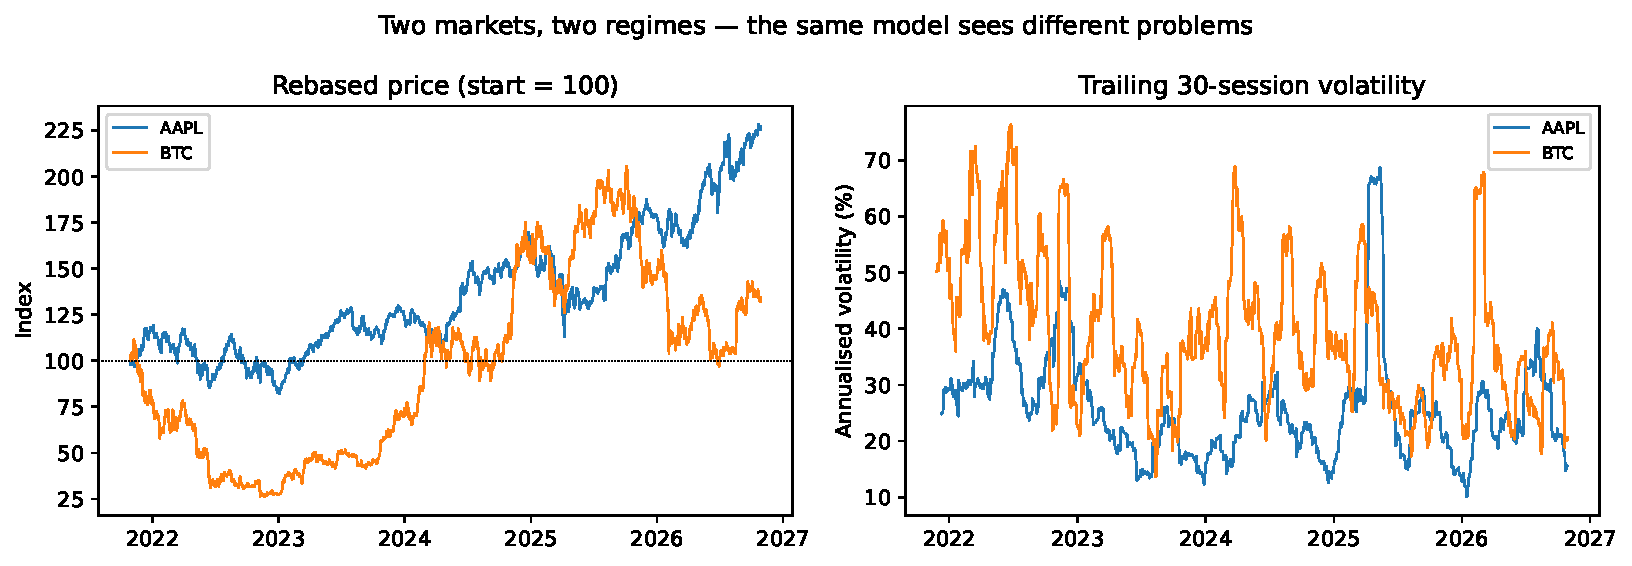
\includegraphics[width=0.9\linewidth]{figures/fig02_asset_characteristics.pdf}
  \caption{How the markets differ. Left: each series rebased to 100. Right:
  annualised 30-session volatility. BTC is usually more volatile.}
  \label{fig:assets}
\end{figure}
